%%%%%
% 
\documentclass[mathserif,graphics]{beamer}
\usepackage{Sweave}
\mode<presentation>
\usetheme{Boadilla} % Beamer Theme
\usecolortheme{whale}
\usepackage{amsmath} % for math AMS fonts
\usepackage{graphicx} % to include figures
\usepackage{subfigure} % to have figures in figures
\usepackage{multimedia} % to include movies

\usepackage[utf8]{inputenc}
\usepackage{amsfonts}
\usepackage{natbib}
\usepackage{scrpage2}
\usepackage{dsfont}
\usepackage{float}
\usepackage{amssymb}

\usepackage{bbm}

\usepackage{tikz}
\usetikzlibrary{arrows,shapes,backgrounds, patterns, decorations.markings} % loads some tikz extensions
\usepackage[english]{babel}
\useoutertheme[subsection=false]{smoothbars} % Beamer Outer Theme
\usepackage{mdframed}
\usepackage{boxedminipage}
\newcommand{\hlcolor}[2]{{\setlength{\fboxsep}{0pt}\colorbox{#1}{\strut #2}}}
\newcommand{\eg}{e.\,g. }
\newcommand{\ie}{i.\,e. }
\newcommand{\cdf}{c.\,d.\,f. }
%\usepackage[usenames,dvipsnames]{xcolor}
\definecolor{lightblue}{rgb}{0.8,0.85,1}


\defbeamertemplate*{footline}{my infolines theme}
    {
      \leavevmode%
      \hbox{%
      \begin{beamercolorbox}[wd=.44\paperwidth,ht=2.25ex,dp=1ex,center]{author
      in head/foot}%
        \usebeamerfont{author in head/foot}\insertshortauthor~~\insertshortinstitute
      \end{beamercolorbox}%
      \begin{beamercolorbox}[wd=.2\paperwidth,ht=2.25ex,dp=1ex,center]{title in
      head/foot}%
        \usebeamerfont{title in head/foot}\insertshorttitle
      \end{beamercolorbox}%
      \begin{beamercolorbox}[wd=.36\paperwidth,ht=2.25ex,dp=1ex,right]{date in
      head/foot}%
        \usebeamerfont{date in head/foot}\insertshortdate{}\hspace*{2em}
        \insertframenumber{} / \inserttotalframenumber\hspace*{2ex}
      \end{beamercolorbox}}%
      \vskip0pt%
    }

\title{Normal Distribution}
%\subtitle{Seminar graph algorithms}
\author{Andrey Chinnov, Sebastian Honermann, Carlos Zydorek}
%\institute{Seminar graph algorithms}
\date{Case Studies \\
"Data Analytics"}

\begin{document}
\frame{
\titlepage
\setbeamercovered{dynamic}
}



\section{Introduction}
\frame{
\frametitle{Outline}
\begin{enumerate}
\item \alert {Introduction}
  \begin{itemize}
  \item Normality as a requirement for statistical methods
  \item Data Set Overview
  \end{itemize}
\item Normality Testing
  \begin{itemize}
  \item Graphical Methods for Normality Testing
    \begin{itemize}
    \item Q-Q-Plots
    \item Chi-Square Plot
    \end{itemize}
  \item Quantitative Methods for Normality Testing
    \begin{itemize}
    \item Shapiro-Wilk Test
    \item Pearson's Chi-Squared Test
    \item Kolmogorov-Smirnov Test
    \end{itemize}
  \end{itemize}
\item Transformation to Normality
  \begin{itemize}
  \item Box-Cox Transformation
  \item Transformation Results Testing 
  \end{itemize}
\item Summary
\end{enumerate}
}
\subsection{Normality as a requirement for statistical methods}

\frame{
\frametitle{Normality as a requirement for statistical methods}

}

\subsection{Data Set Overview}

\frame{
\frametitle{Data Set Overview}

}

\section{Normality Testing}
\frame{
\frametitle{Outline}
\begin{enumerate}
\item Introduction
  \begin{itemize}
  \item Normality as a requirement for statistical methods
  \item Data Set Overview
  \end{itemize}
\item \alert{Normality Testing}
  \begin{itemize}
  \item Graphical Methods for Normality Testing
    \begin{itemize}
    \item Q-Q-Plots
    \item Chi-Square Plot
    \end{itemize}
  \item Quantitative Methods for Normality Testing
    \begin{itemize}
    \item Shapiro-Wilk Test
    \item Pearson's Chi-Squared Test
    \item Kolmogorov-Smirnov Test
    \end{itemize}
  \end{itemize}
\item Transformation to Normality
  \begin{itemize}
  \item Box-Cox Transformation
  \item Transformation Results Testing 
  \end{itemize}
\item Summary
\end{enumerate}
}

\subsection{Q-Q-Plots}
\frame{
\frametitle{Graphical Methods for Normality Testing}
\framesubtitle{Q-Q-Plots}
}

\subsection{Chi-Square Plot}
\frame{
\frametitle{Graphical Methods for Normality Testing}
\framesubtitle{Chi-Square Plot}
}

\subsection{Shapiro-Wilk Test}
\frame{
\frametitle{Quantitative Methods for Normality Testing}
\framesubtitle{Shapiro-Wilk Test}
}

\subsection{Pearson's Chi-Squared Test}
\frame{
\frametitle{Quantitative Methods for Normality Testing}
\framesubtitle{Pearson's Chi-Squared Test}
}

\subsection{Kolmogorov-Smirnov Test}
\frame{
\frametitle{Quantitative Methods for Normality Testing}
\framesubtitle{Kolmogorov-Smirnov Test}
Let $x=(x_1,x_2, \dots, x_n)$ be a sample of a given size $n$.
\begin{columns}[t]
\column{0.5\columnwidth}
\begin{definition}
$F_n=\frac{1}{n}\sum_{i=1}^n \mathbbm{1}_{\{x_i\le x\}}$ - empirical
\cdf, where $\forall  x\in \mathbb{R}$ $\mathbbm{1}_{\{x_i\le x\}}(x)=\left\lbrace 
\begin{array}{cll}
                1 & \mbox{if} \ x_i\le x\\
                 0 & \mbox{otherwise}.
\end{array} 
\right.$
\end{definition}
\column{0.5\columnwidth}
  \vspace{-1cm}
    \begin{figure}
	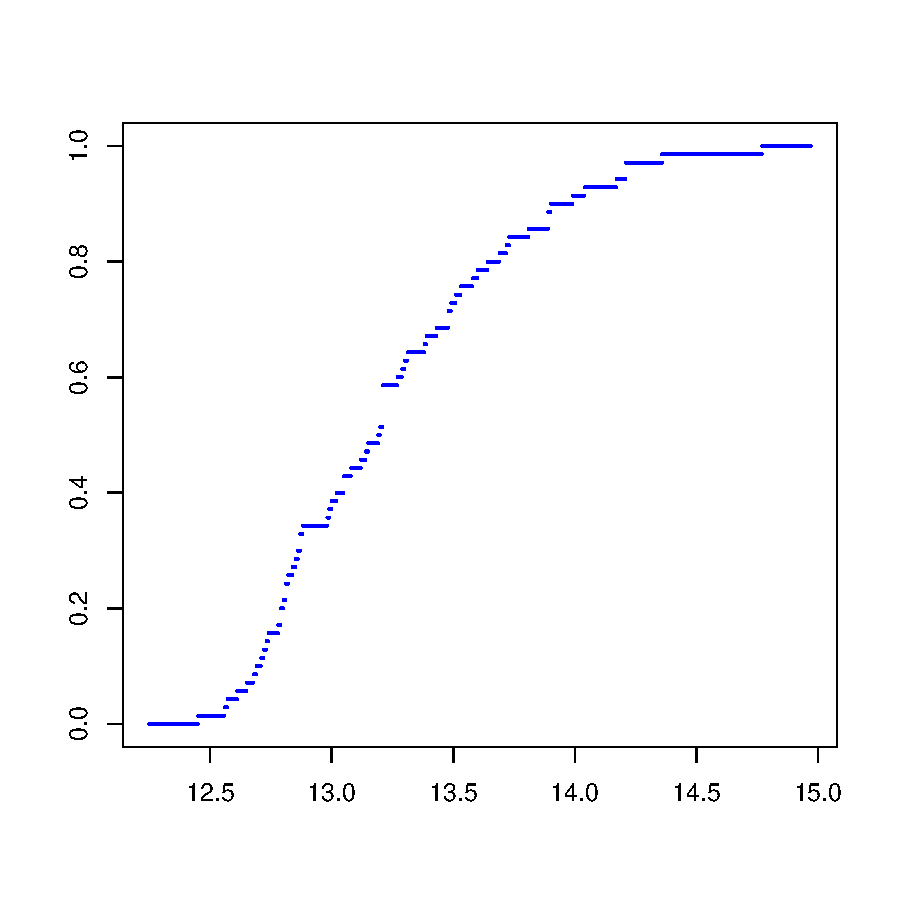
\includegraphics[width=\columnwidth]{Report-empiricFunc}
	\end{figure}
\vspace{-1.5cm}
\begin{center}
Glass Type 1, Natrium (Na)
\end{center}
\end{columns}



}


\section{Transformation to Normality}
\frame{
\frametitle{Outline}
\begin{enumerate}
\item Introduction
  \begin{itemize}
  \item Normality as a requirement for statistical methods
  \item Data Set Overview
  \end{itemize}
\item Normality Testing
  \begin{itemize}
  \item Graphical Methods for Normality Testing
    \begin{itemize}
    \item Q-Q-Plots
    \item Chi-Square Plot
    \end{itemize}
  \item Quantitative Methods for Normality Testing
    \begin{itemize}
    \item Shapiro-Wilk Test
    \item Pearson's Chi-Squared Test
    \item Kolmogorov-Smirnov Test
    \end{itemize}
  \end{itemize}
\item \alert{Transformation to Normality}
  \begin{itemize}
  \item Box-Cox Transformation
  \item Transformation Results Testing 
  \end{itemize}
\item Summary
\end{enumerate}
}
\subsection{Box-Cox Transformation}

\frame{
\frametitle{Box-Cox Transformation}

}

\subsection{Transformation Results Testing}

\frame{
\frametitle{Transformation Results Testing}

}

\section{Summary}
\frame{
\frametitle{Outline}
\begin{enumerate}
\item Introduction
  \begin{itemize}
  \item Normality as a requirement for statistical methods
  \item Data Set Overview
  \end{itemize}
\item Normality Testing
  \begin{itemize}
  \item Graphical Methods for Normality Testing
    \begin{itemize}
    \item Q-Q-Plots
    \item Chi-Square Plot
    \end{itemize}
  \item Quantitative Methods for Normality Testing
    \begin{itemize}
    \item Shapiro-Wilk Test
    \item Pearson's Chi-Squared Test
    \item Kolmogorov-Smirnov Test
    \end{itemize}
  \end{itemize}
\item Transformation to Normality
  \begin{itemize}
  \item Box-Cox Transformation
  \item Transformation Results Testing 
  \end{itemize}
\item \alert{Summary}
\end{enumerate}
}
\subsection{Summary}
\frame{
\frametitle{Summary}
}

\end{document}
